
\section{Task 1 - Maximum Likelihood Estimation}



\subsection*{1.1 Derivation}

Likelihood of a single sample of dimension m:

$$
p(x|\theta) = \frac{1}{\sqrt{(2 \pi )^3 \vert \Sigma \vert}} e^{-\frac{1}{2} (x-\mu )^T \Sigma ^{-1} (x-\mu)}
$$

Likelihood for a set X of N samples:

$$
X = \{x_1, x_2 .. x_N\}
$$


$$
p(X|\theta) = \prod_{i=1}^{N} \frac{1}{\sqrt{(2 \pi )^3 \vert \Sigma \vert}} e^{-\frac{1}{2} (x_i-\mu )^T \Sigma ^{-1} (x_i-\mu)}
$$



$$
\vert \Sigma \vert = \sigma^6
$$


Add logarithms to both sides of the equation to obtain log-likelihood:
$$
log(p(X|\theta)) = \sum_{i=1}^{N}log(\frac{1}{\sqrt{(2 \pi )^3 \vert \Sigma \vert}} e^{-\frac{1}{2} (x_i-\mu )^T \Sigma ^{-1} (x_i-\mu)})
$$

$$
log(p(X|\theta)) = \sum_{i=1}^{N} log(\frac{1}{\sqrt{(2 \pi )^3 \vert \Sigma \vert}}) + log( e^{-\frac{1}{2} (x_i-\mu )^T \Sigma ^{-1} (x_i-\mu)})
$$

$$
log(p(X|\theta)) = \sum_{i=1}^{N} log(\frac{1}{\sqrt{(2 \pi )^3 \vert \Sigma \vert}})  {-\frac{1}{2} (x_i-\mu )^T \Sigma ^{-1} (x_i-\mu)}
$$





$$
(x_i-\mu )^T \Sigma ^{-1} (x_i-\mu) = (x_i-\mu )^T \sigma^{-2} I ^{-1} (x_i-\mu) = \sigma^{-2} (x_i-\mu )^T (x_i-\mu)
$$


Inner product given by:
$$
(x_i-\mu )^T  (x_i-\mu) = \sum_{j=1}^{m} (x_{i,j} - \mu_{i,j})^2
$$

\subsection*{1.2 Finding the Maximum}

For finding the maximum likelihood estimation of $\mu$, the log-likelihood is derived wrt. the different vector components of $\mu$, and then set to zero. Since the log-expression is monotonically increasing and without upper bound, a root in the derivative of the expression must be corresponding to a minimum in the log function, and therefore a minimum in the original likelihood function. This is because a monotonic function without upper bounds like the likelihood function does not have maxima. The addition of logarithms does not alter the function in terms of locations of its extrema.
In the following, the derivation is carried out for component j, which is one component of the m-dimensional data.

$$
\frac{dlog(p(X|\theta))}{d\mu_j} = -\frac{1}{2\sigma^2}    \sum_{i=1}^{N}    \frac{d}{d\mu_j}
(x_{i,j} - \mu_{j})^2 
$$


$$
\frac{dlog(p(X|\theta))}{d\mu_j} = -\frac{1}{2\sigma^2}    \sum_{i=1}^{N}    \frac{d}{d\mu_j}
(x_{i,j}^2 - 2 x_{i,j} \mu_{j} + \mu_{j}^2 ) 
$$


$$
\frac{dlog(p(X|\theta))}{d\mu_j} = -\frac{1}{\sigma^2}    \sum_{i=1}^{N}   (- x_{i,j}  +  \mu_{j} ) 
$$




$$
\frac{dlog(p(X|\theta))}{d\mu_j} = -\frac{1}{\sigma^2}    \sum_{i=1}^{N}   (- x_{i,j})  +  N\mu_{j}  \musteq 0
$$

Finally giving the maximum likelihood estimation for $\mu$, which is just the mean value of component $j$ of samples $x_i$ in the set:

$$
\mu_{j}  =   \frac{1}{N} \sum_{i=1}^{N}   (x_{i,j})
$$



\section{Task 2 - Practical: Selecting data and coding}
\subsection{Selecting data}


The first task of the practical is to choose a dataset, and from that choose 3 metrics that are reasonably close to be normal distributed. 
The chosen dataset is 'social\_capital\_zip.csv'.

To make a quick assesment about the distribution of the underlying distribution of different metrics provided in the raw data, histogram plots are created. These plots show the dnumber of datapoints in a umber of bins, after the raw data has been binned according to lower and upper bound of the individual bins. There are many metrics in the raw data that do not at all follow a gaussian distribution. Many metrics, most notably the pop\_2018 metric, seem to follow Benfords law (as we should expect), which is very much skewed towards low population values, shown in figure \ref{fig:fig_pop_2018}






\begin{figure}[H]
	\centering
	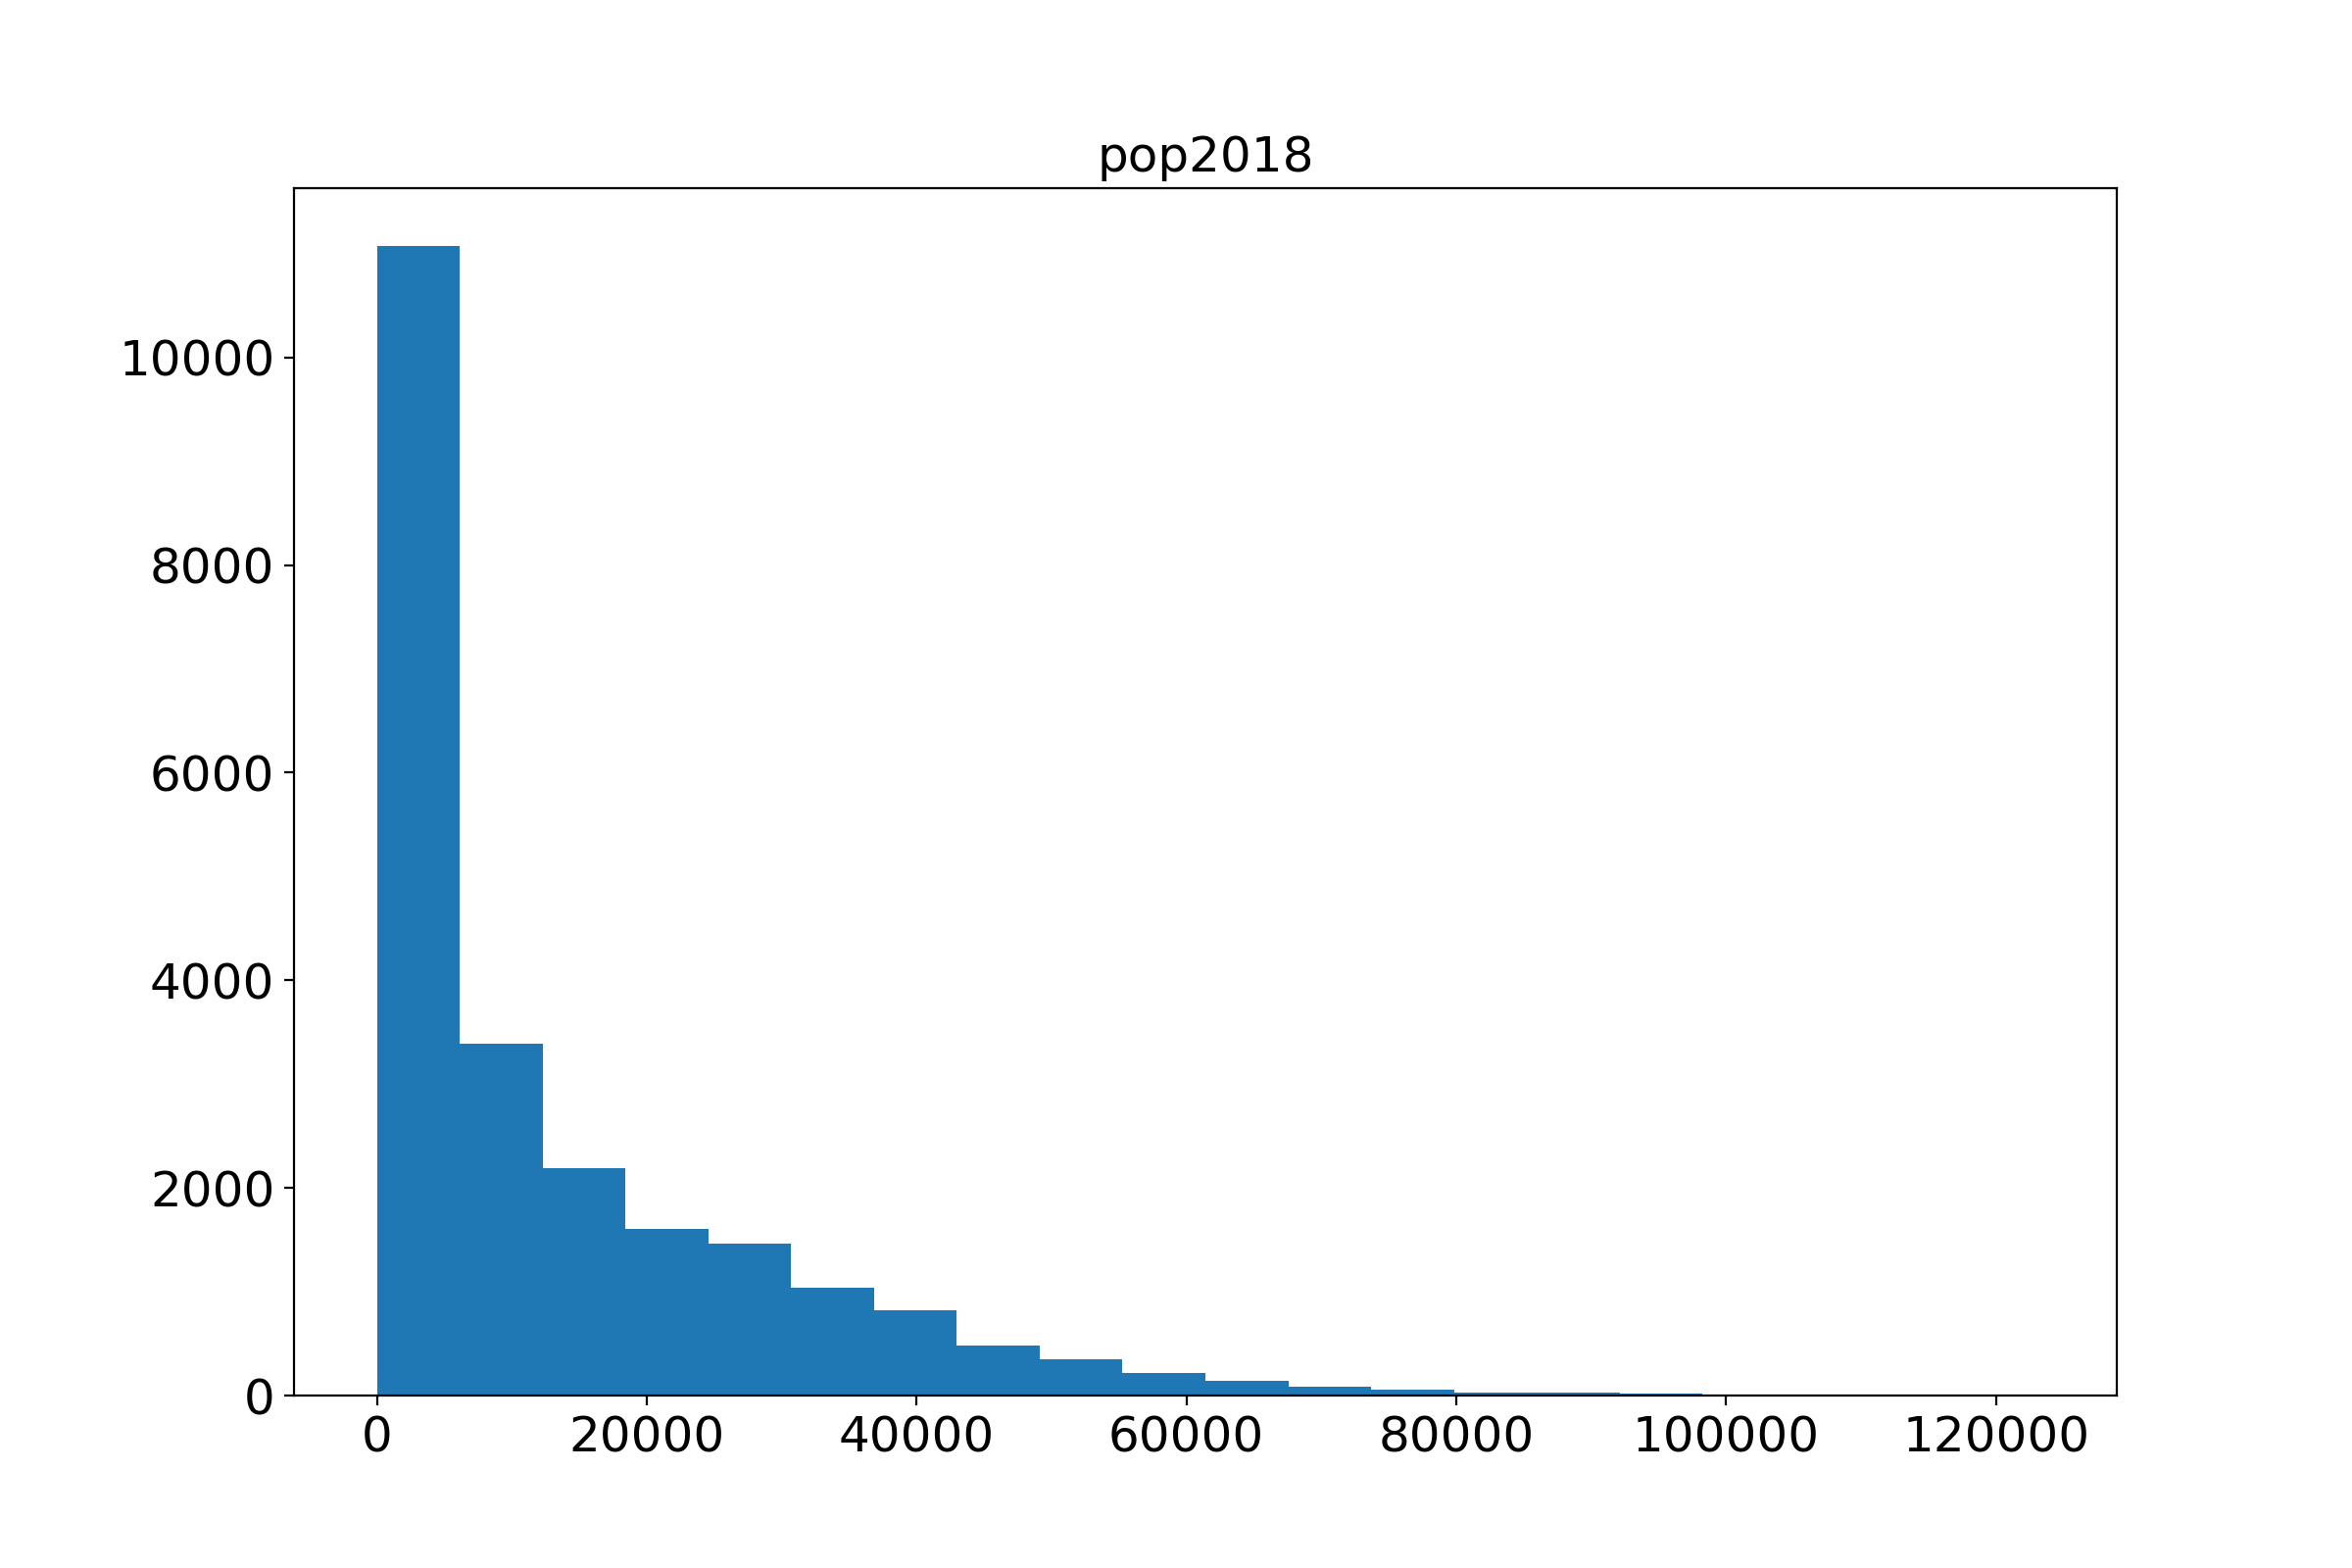
\includegraphics[width=0.9\linewidth]{images/pop2018_hist.png}
	\caption{Population in the year 2018 appears to follow Benford's law}
	\label{fig:fig_pop_2018}
\end{figure}


After a bit of trial and error, the metrics "exposure\_grp\_mem\_zip", "nbhd\_ec\_zip" and "bias\_grp\_mem\_zip" were chosen, with their distributions shown in figure \ref{fig:fig_bias_grp_mem_zip_hist}, \ref{fig:fig_exposure_grp_mem_zip_hist} and \ref{fig:fig_nbhd_ec_zip_hist}:




\begin{figure}[H]
	\centering
	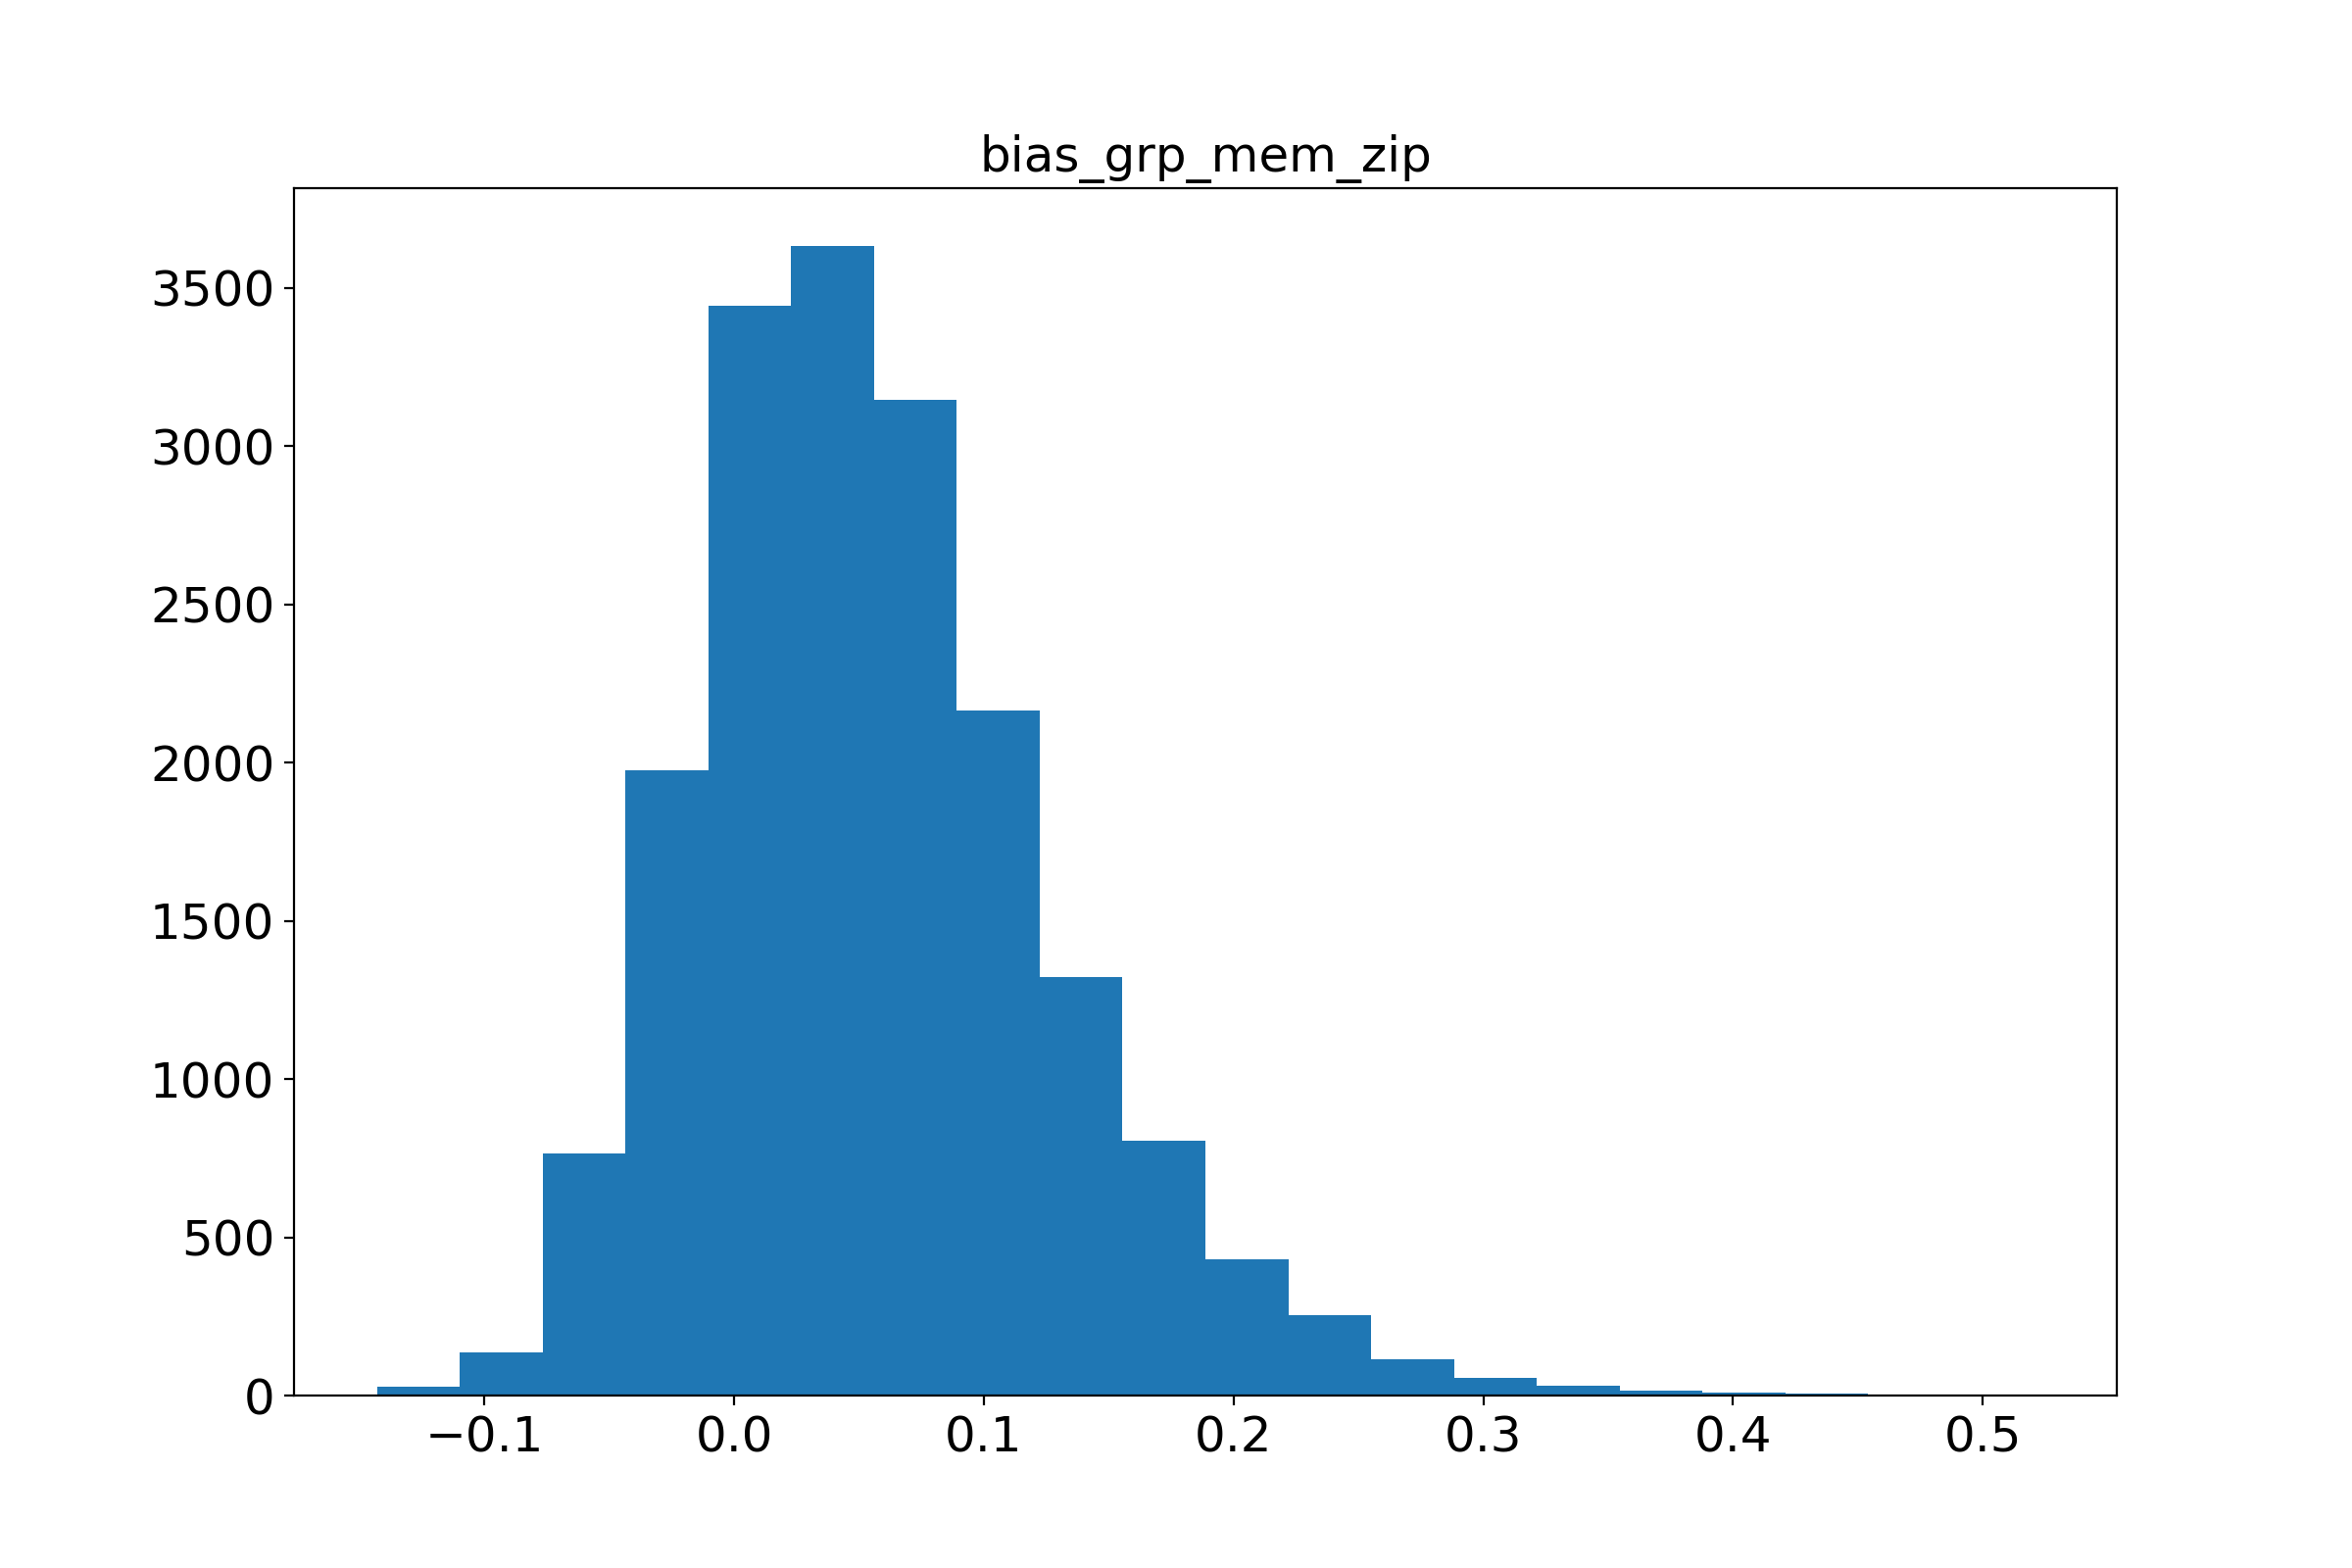
\includegraphics[width=0.9\linewidth]{images/bias_grp_mem_zip_hist.png}
	\caption{Size of bias groups}
	\label{fig:fig_bias_grp_mem_zip_hist}
\end{figure}




\begin{figure}[H]
	\centering
	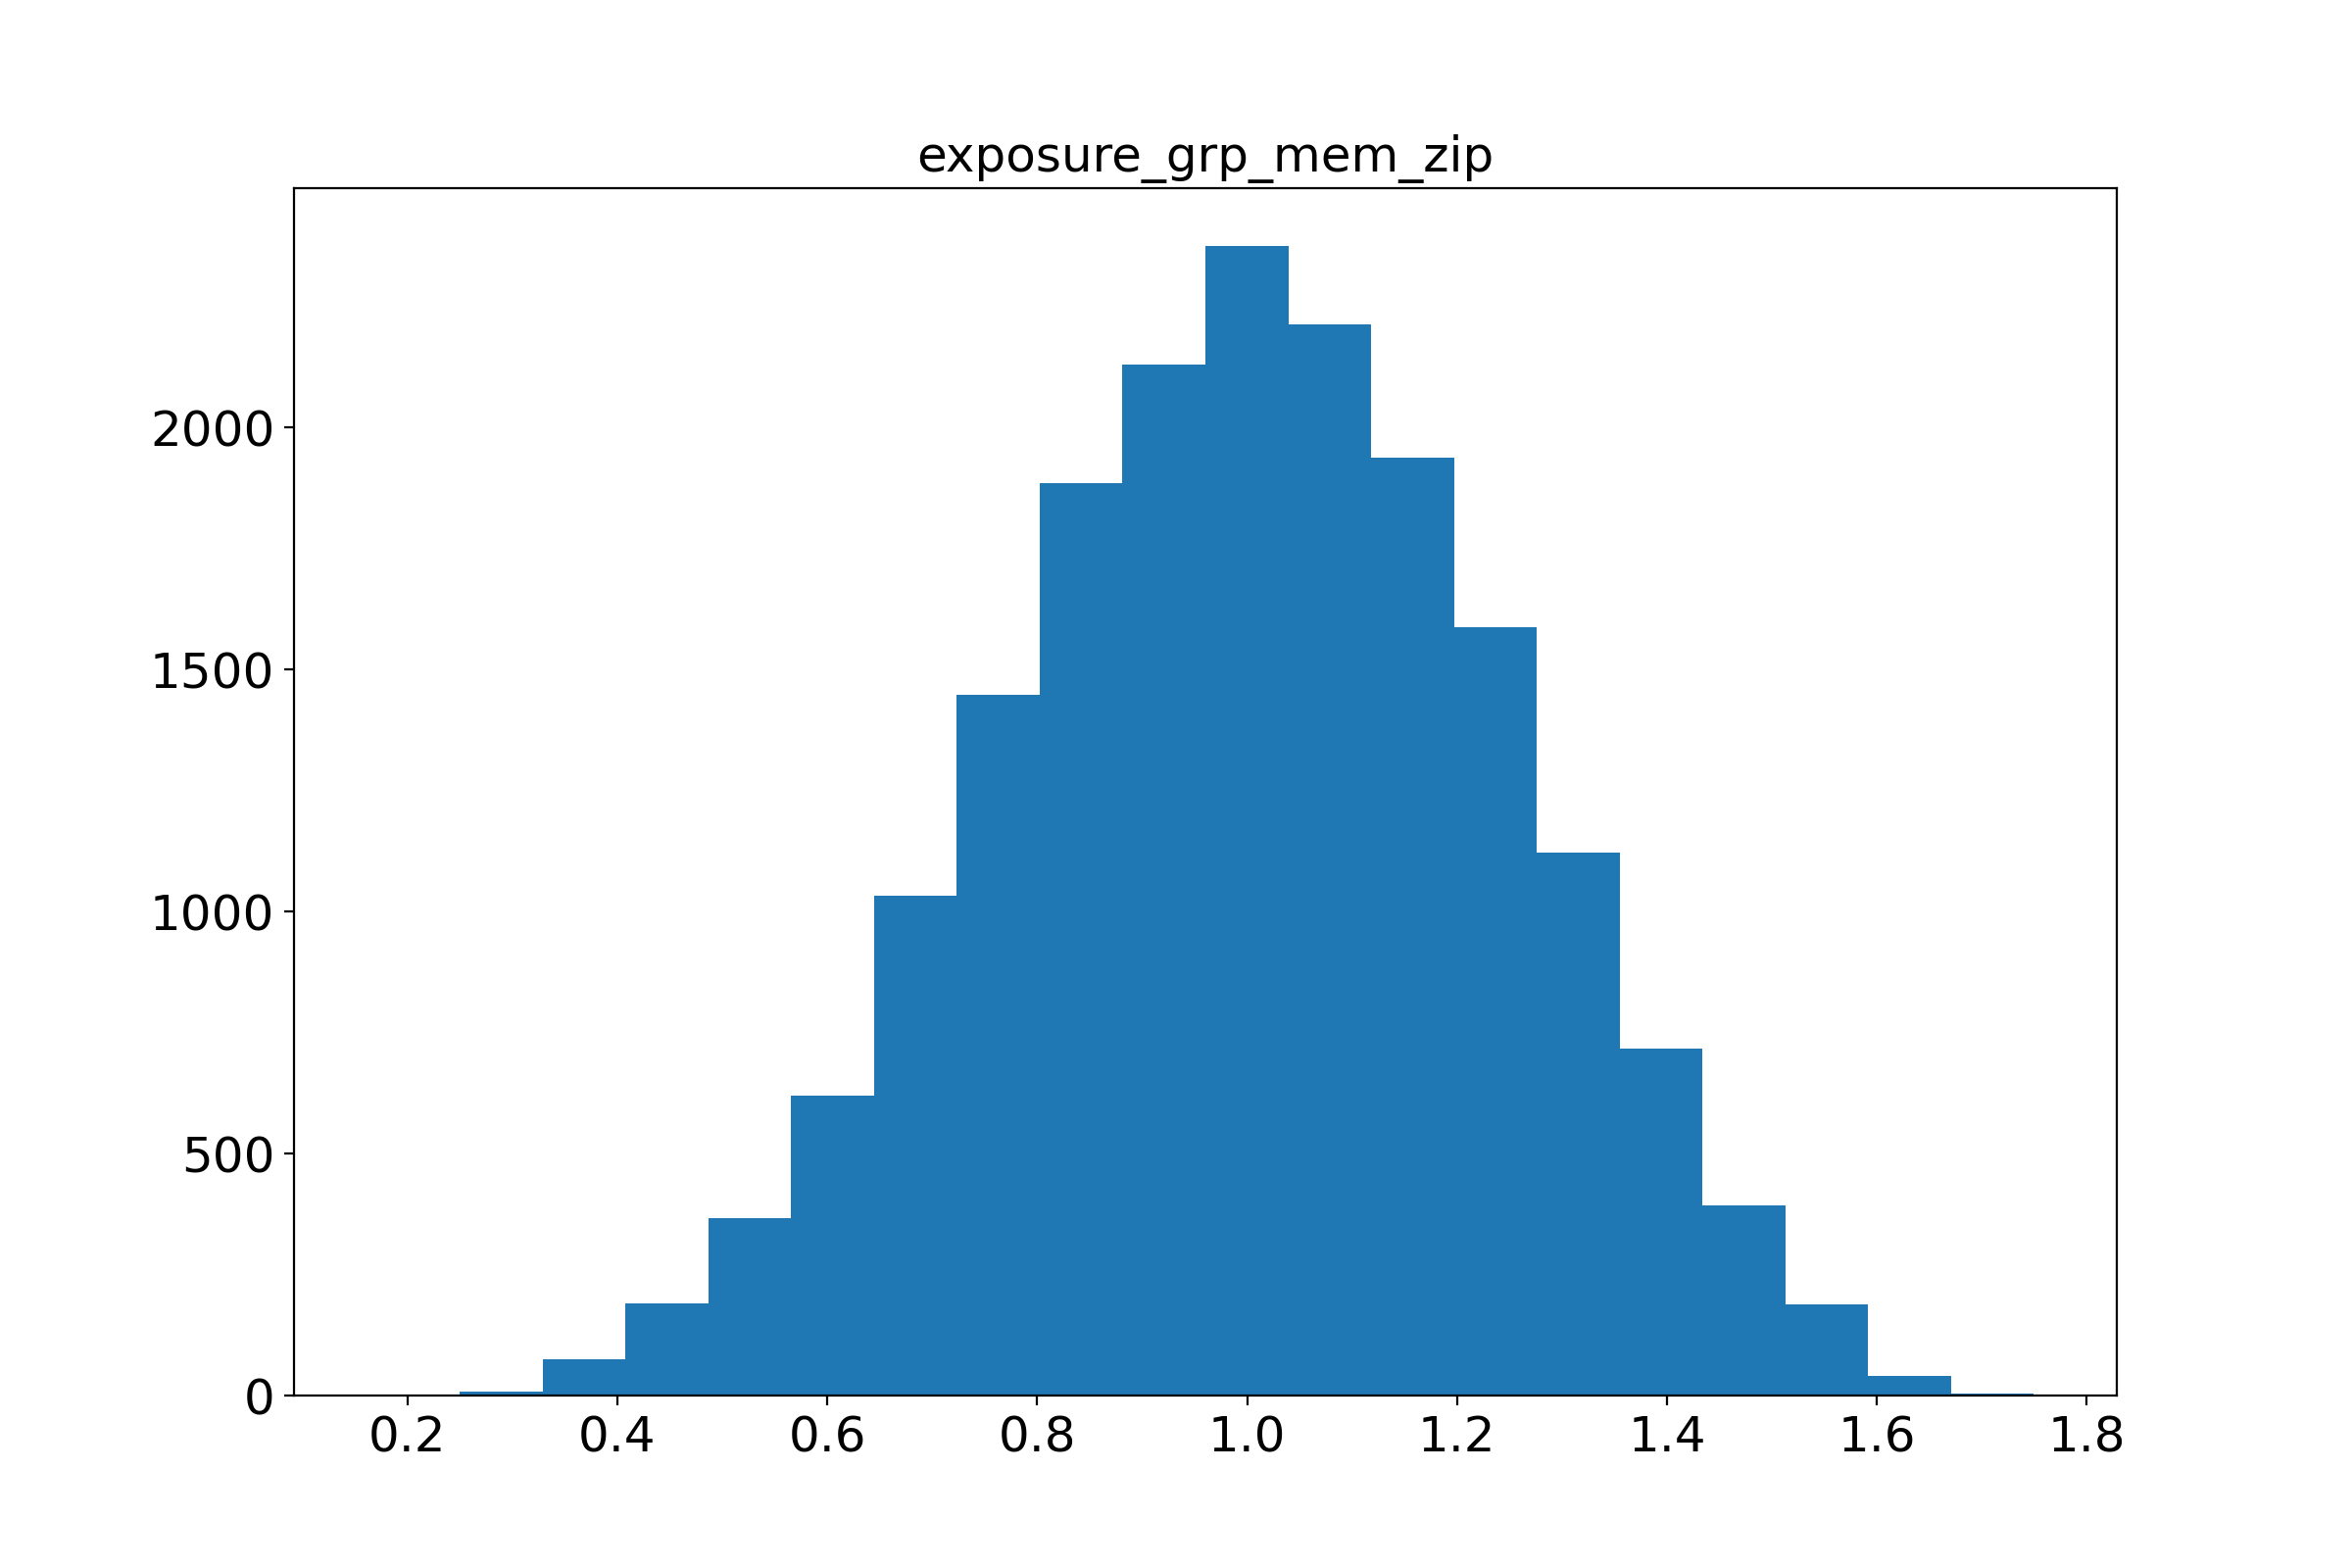
\includegraphics[width=0.9\linewidth]{images/exposure_grp_mem_zip_hist.png}
	\caption{Mean exposure to high-SES individuals by ZIP code for low-SES individuals}
	\label{fig:fig_exposure_grp_mem_zip_hist}
\end{figure}




\begin{figure}[H]
	\centering
	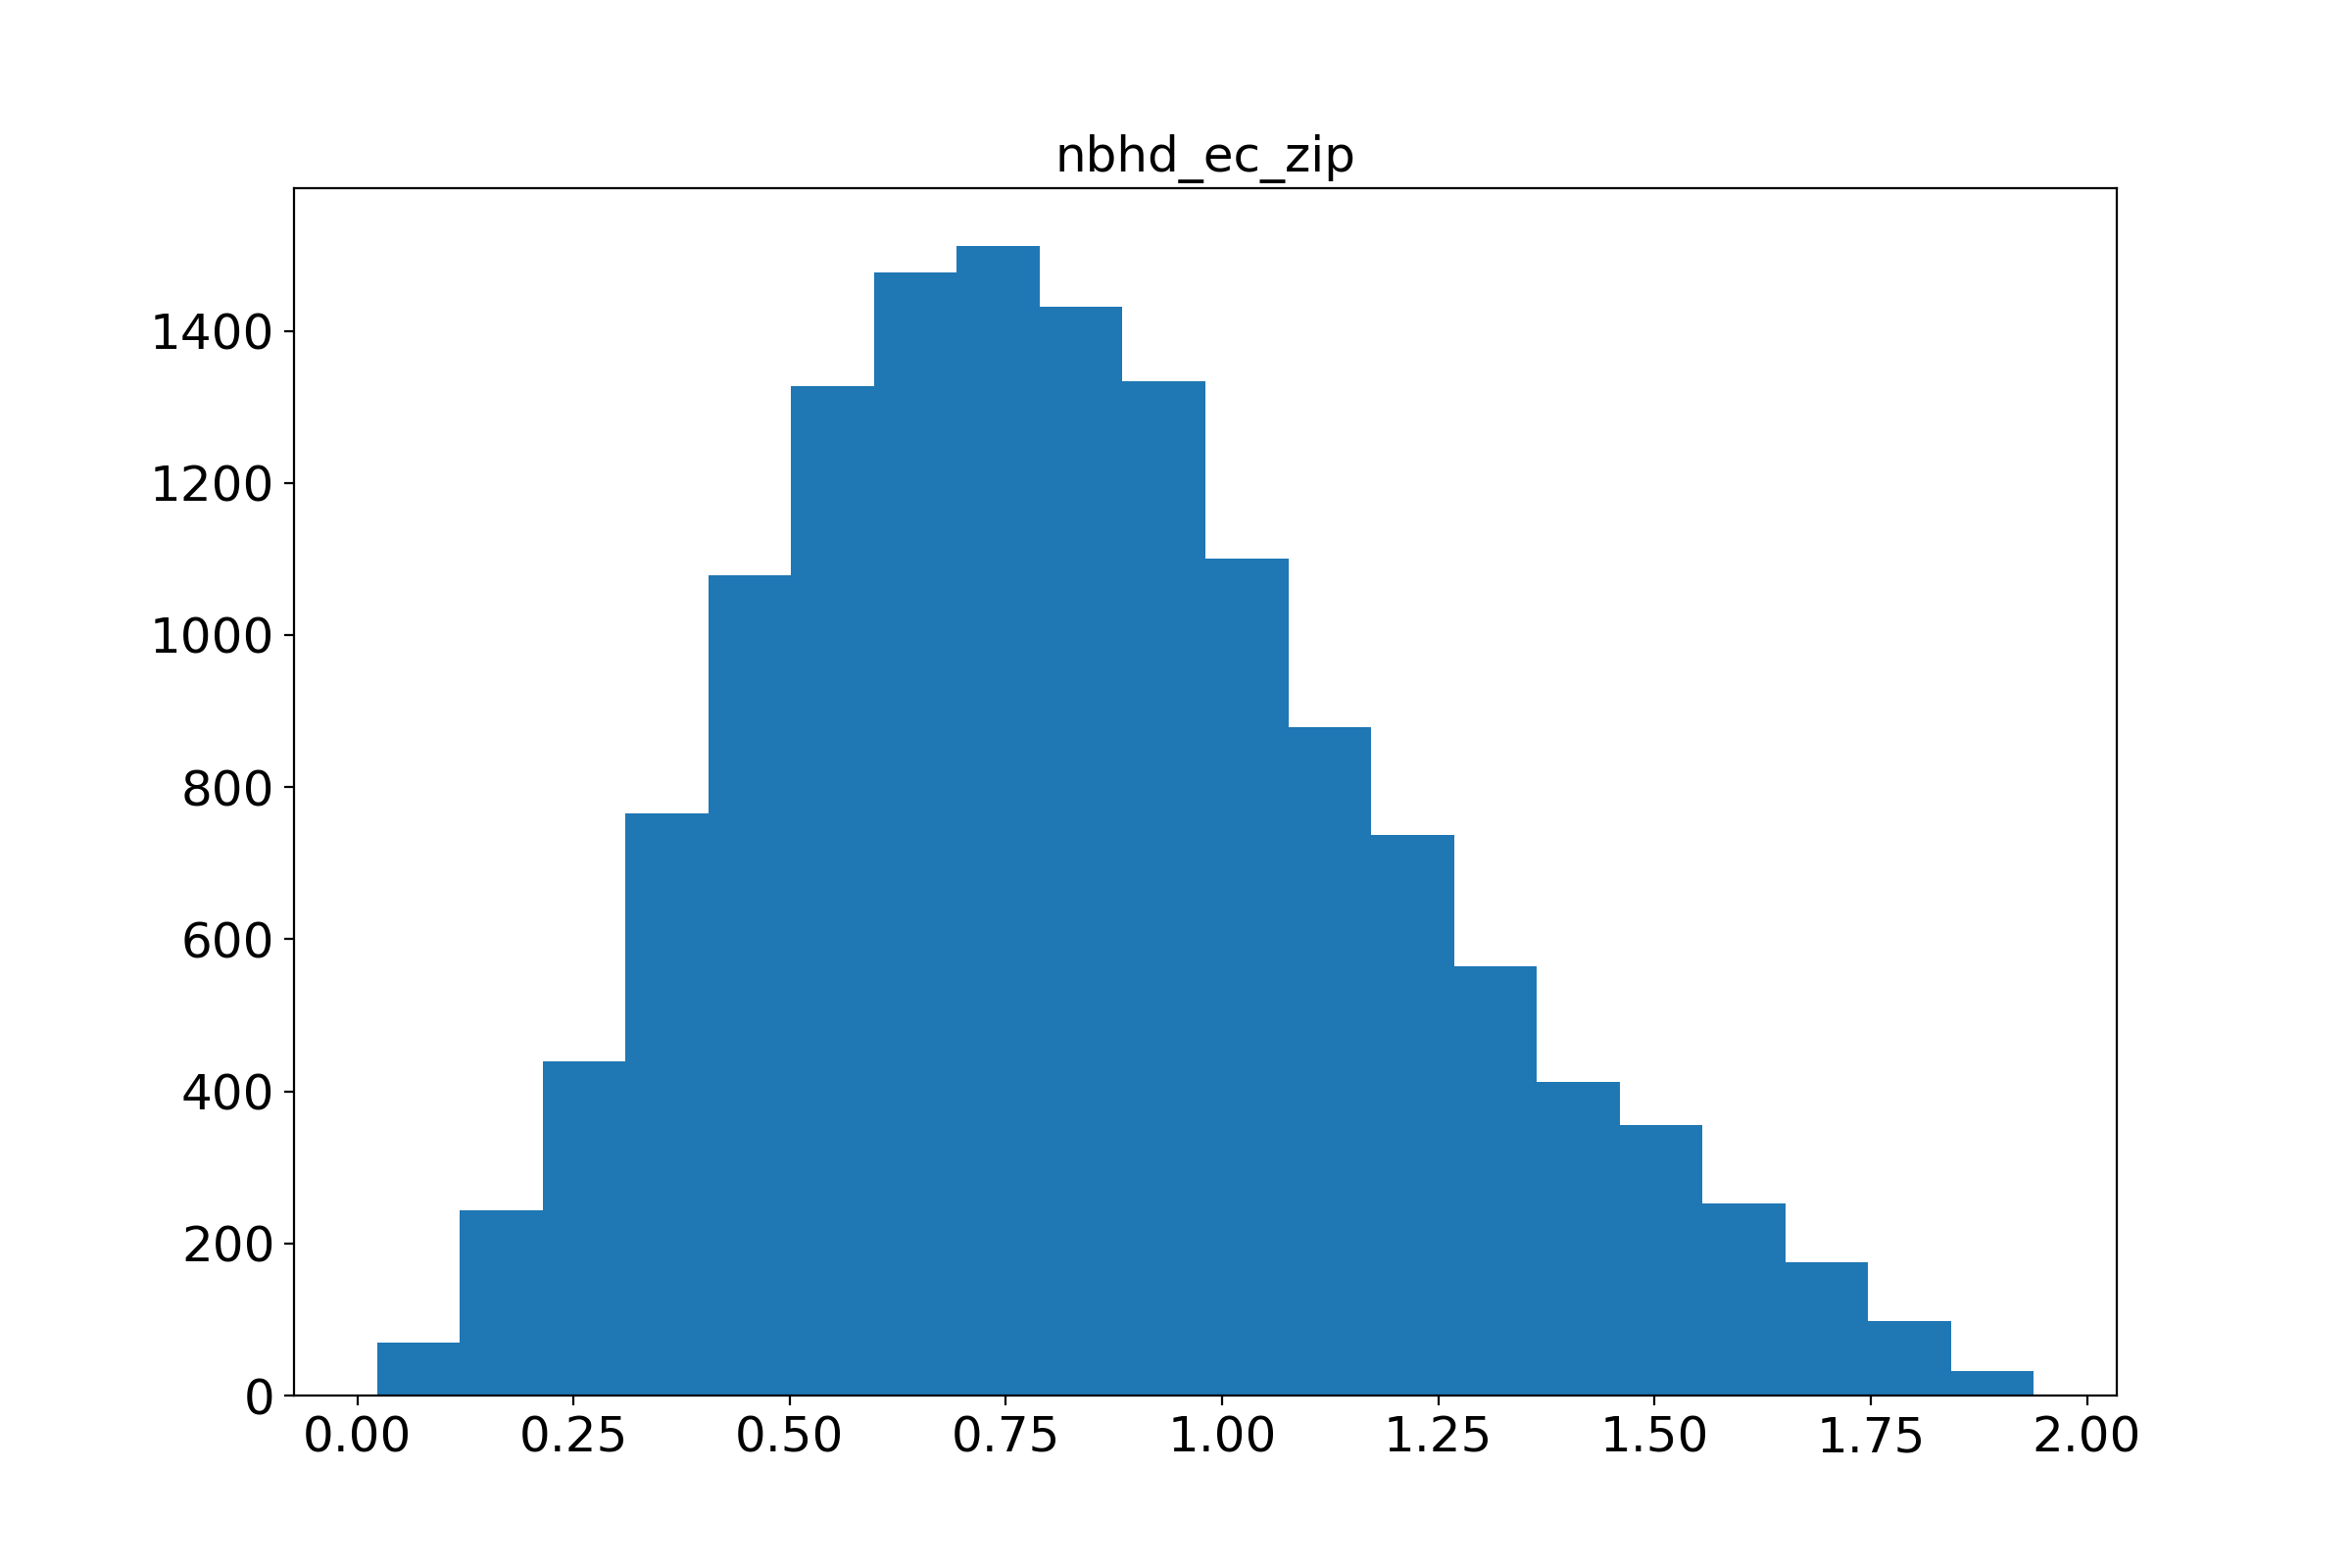
\includegraphics[width=0.9\linewidth]{images/nbhd_ec_zip_hist.png}
	\caption{ec grp mem zip divided by exposure grp mem zip, all subtracted from one}
	\label{fig:fig_nbhd_ec_zip_hist}
\end{figure}



To test if the three individual dataseries combine to a 3D gaussian distribution, we create a 3D scatter-plot and assess the qualitative appearance in figure \ref{fig:fig_3Dscatter}:


\begin{figure}[H]
	\centering
	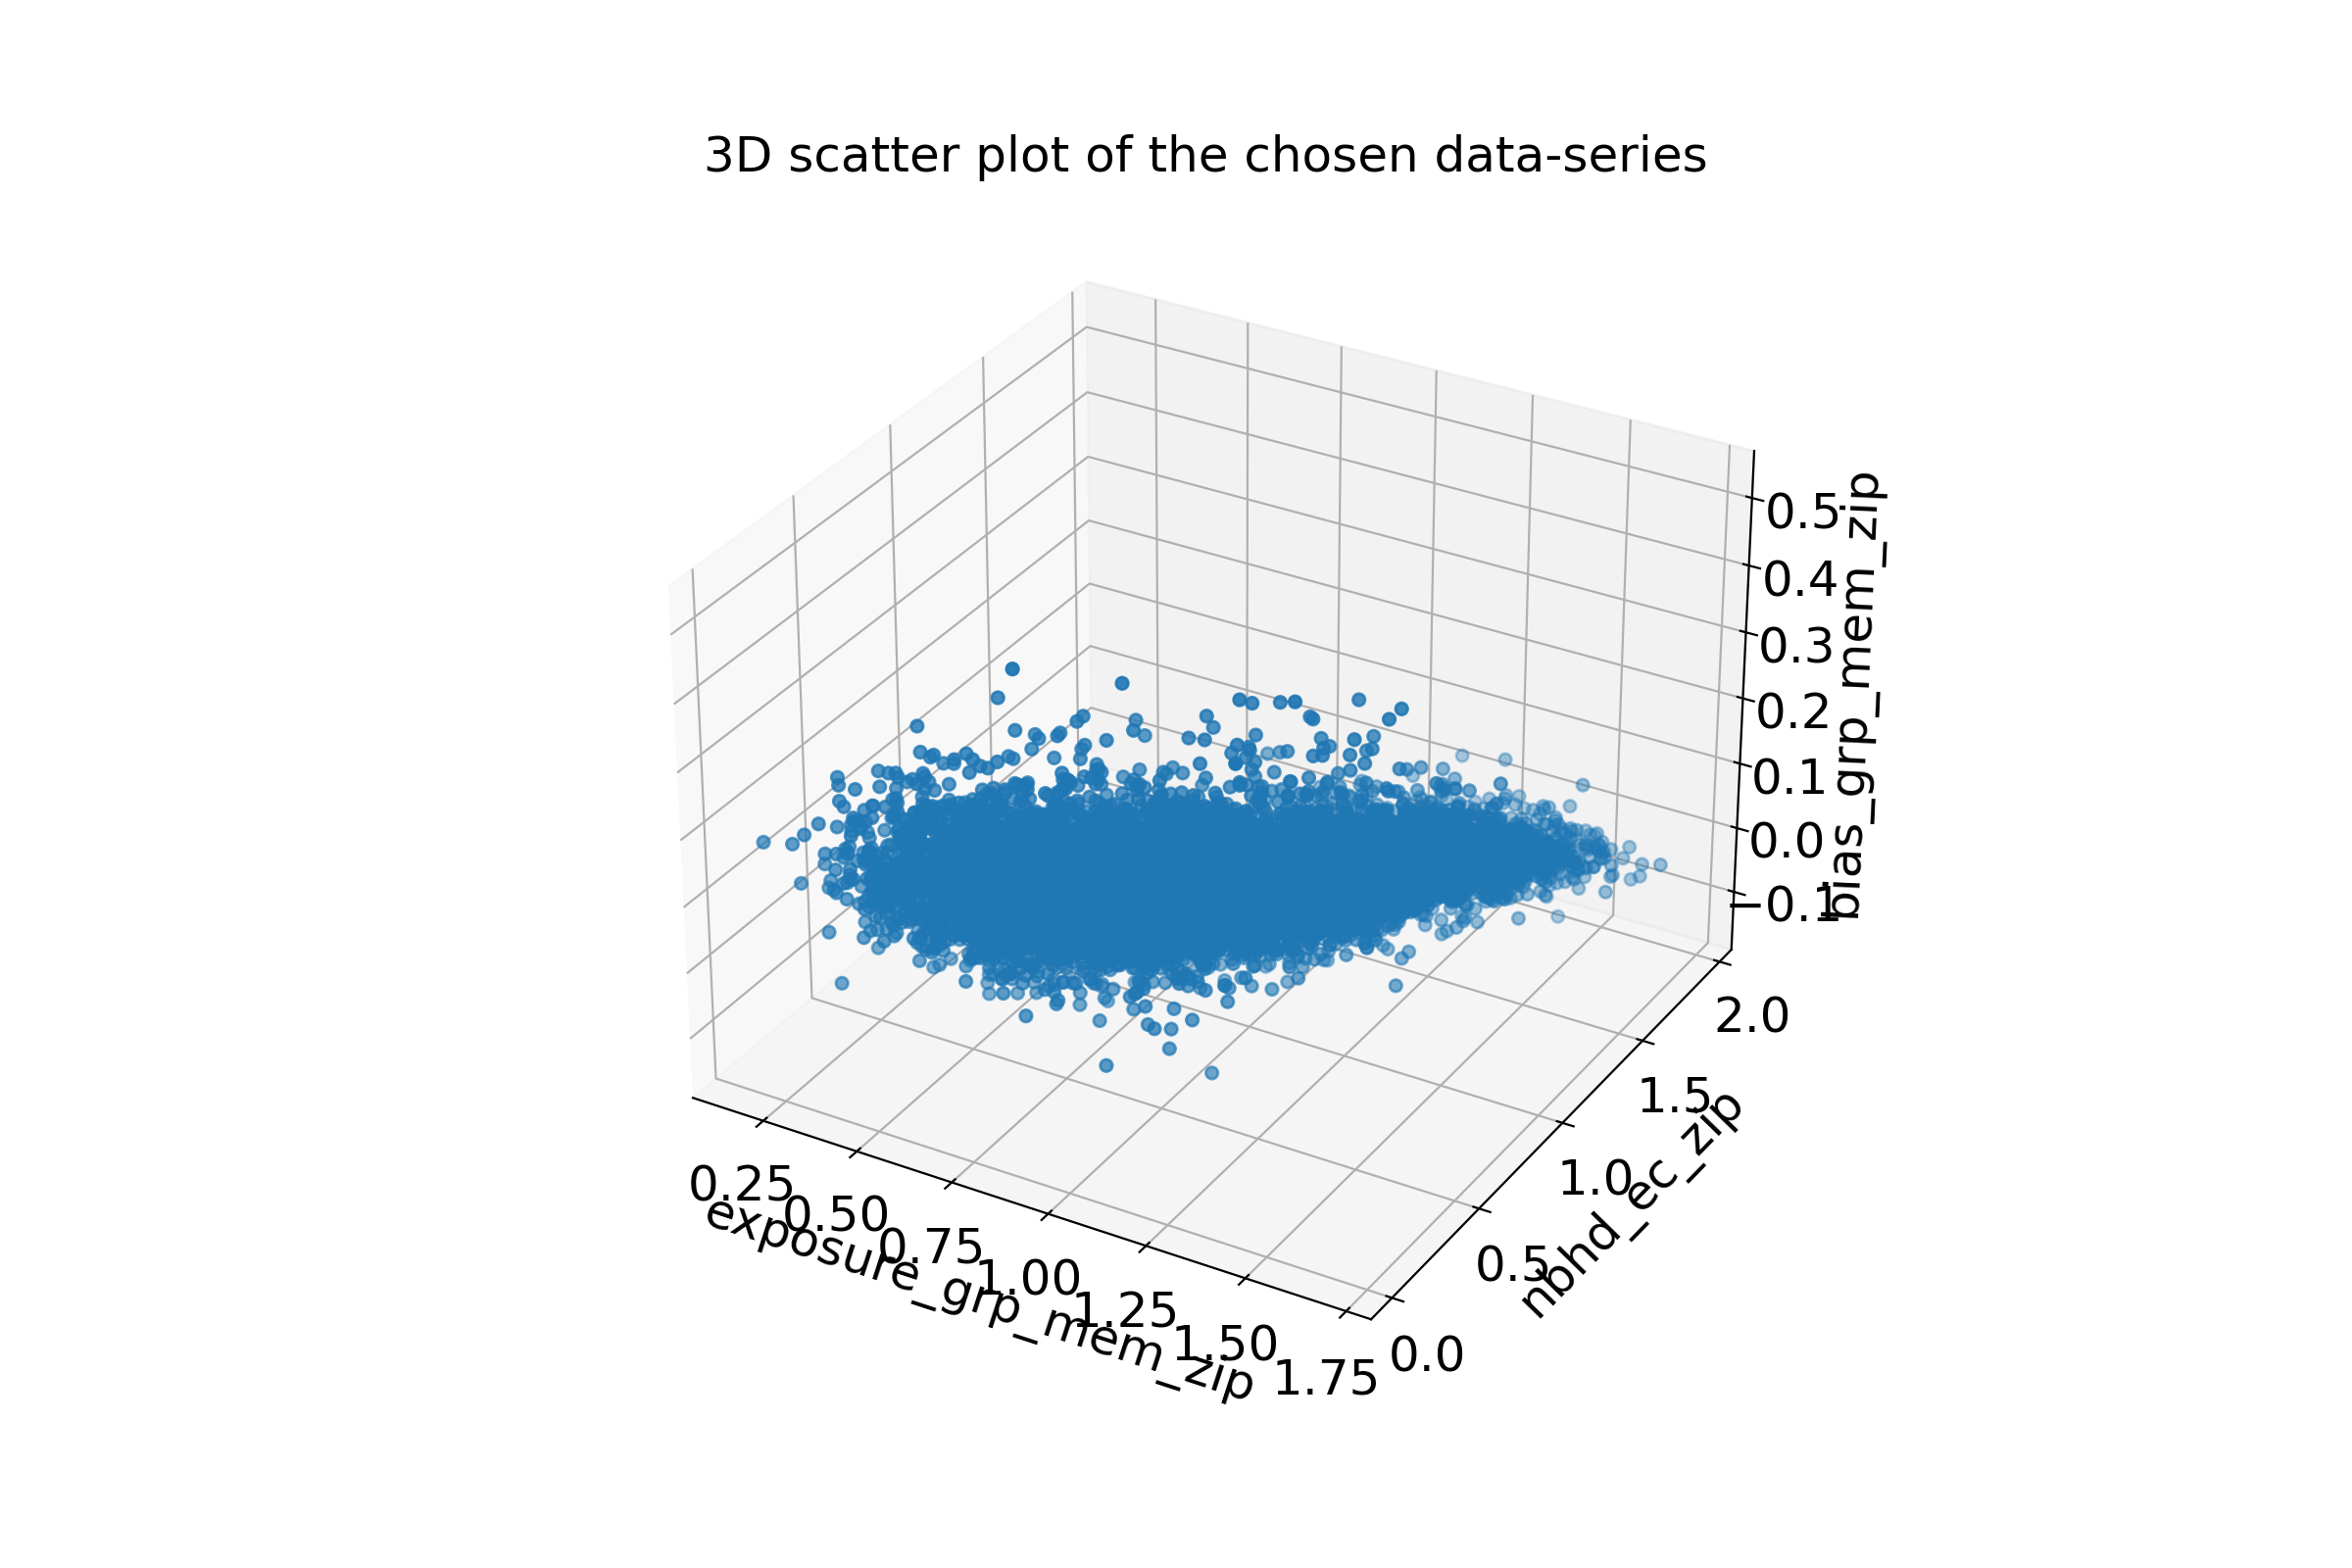
\includegraphics[width=0.9\linewidth]{images/3Dscatter.png}
	\caption{3D scatter plot of the chosen metrics}
	\label{fig:fig_3Dscatter}
\end{figure}


The 3D scatter plot creates a point cloud in 3D space that appears to be reasonably well distributed without much skewing towards one area or without exhibiting multiple clusters. The chosen metrics appear to satisfy the requirements given in the task description.

\subsection{Calculating the maximum likelihood estimation of $\mu$}
Finally, the maximum likelihood estimation is calculated as the mean of the three dataseries, giving the vector:

$$
\bf{\mu} = 
	\begin{bmatrix}
	\mu_{egm} \\
	\mu_{nbhd\_ec} \\
	\mu_{bgm} \\
	\end{bmatrix}  =
	\begin{bmatrix}
	1.005 \\
	0.839 \\
	0.057
\end{bmatrix}
$$




















